We generate three types of graphs from the attached code. The first series, shown below show the evolution of the probability distribution, as the means and covariance matrices are updated.\\
% 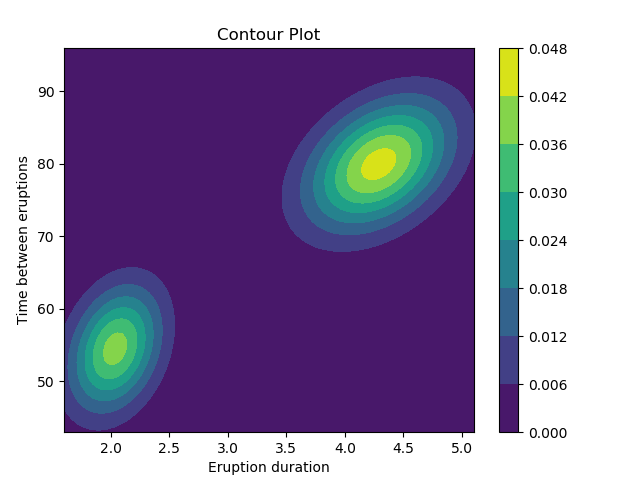
\includegraphics[width=0.5\linewidth]{contour.png}
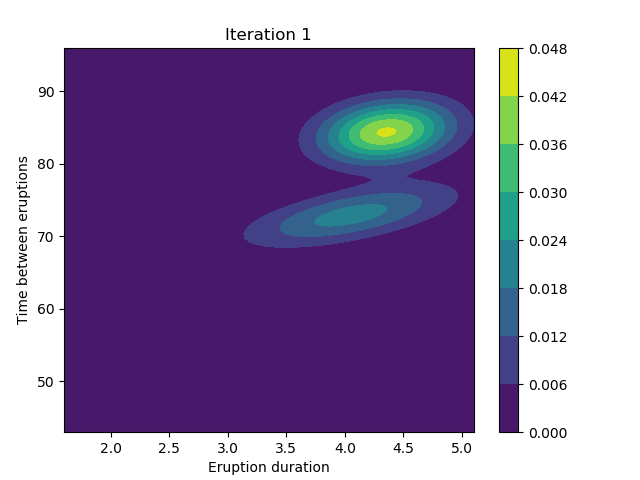
\includegraphics[width=0.33\linewidth]{contour1.png}
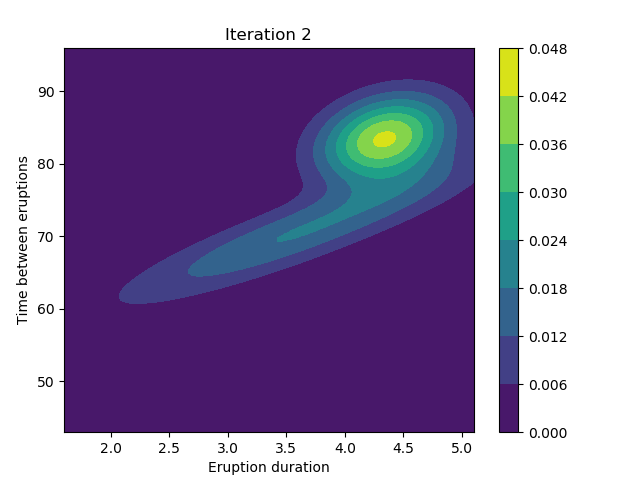
\includegraphics[width=0.33\linewidth]{contour2.png}
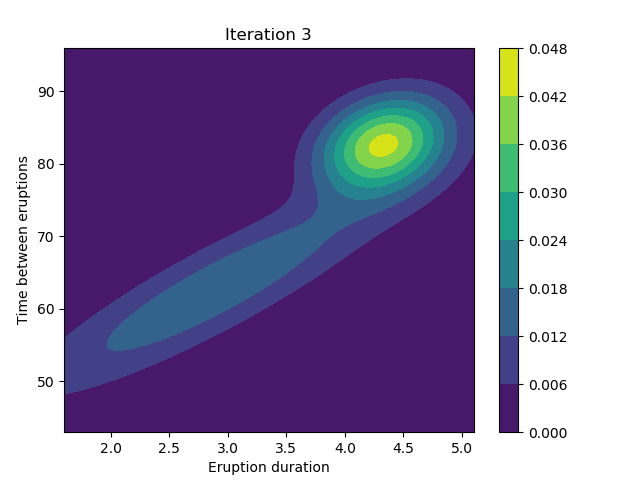
\includegraphics[width=0.33\linewidth]{contour3.png}
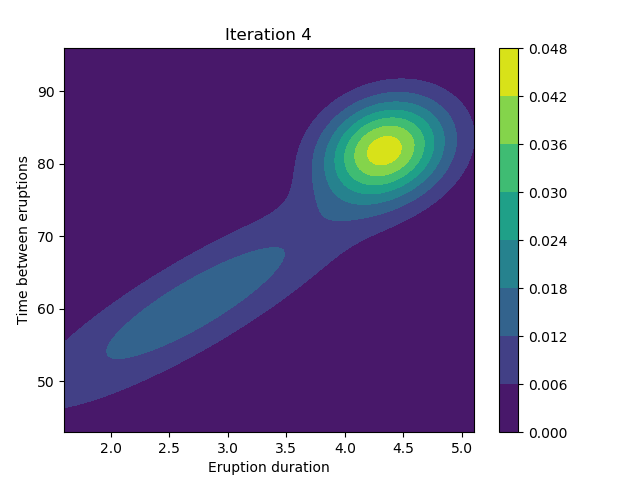
\includegraphics[width=0.33\linewidth]{contour4.png}
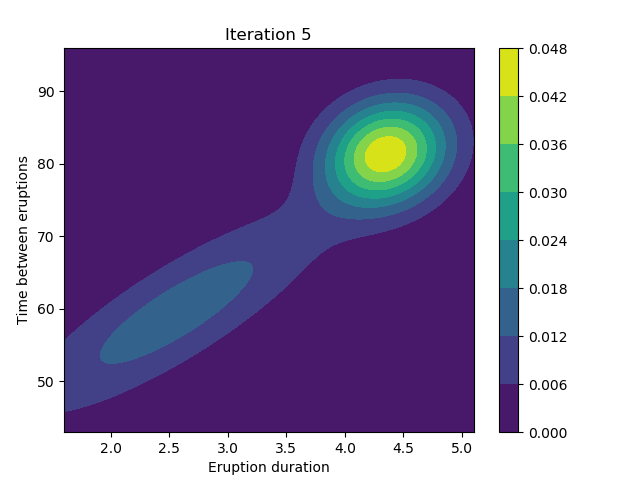
\includegraphics[width=0.33\linewidth]{contour5.png}
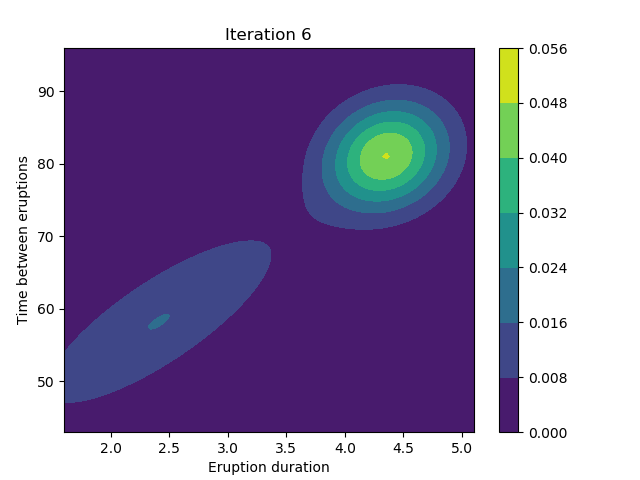
\includegraphics[width=0.33\linewidth]{contour6.png}
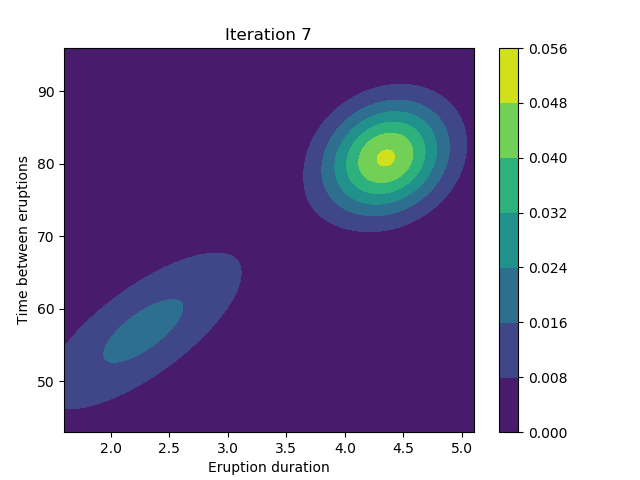
\includegraphics[width=0.33\linewidth]{contour7.png}
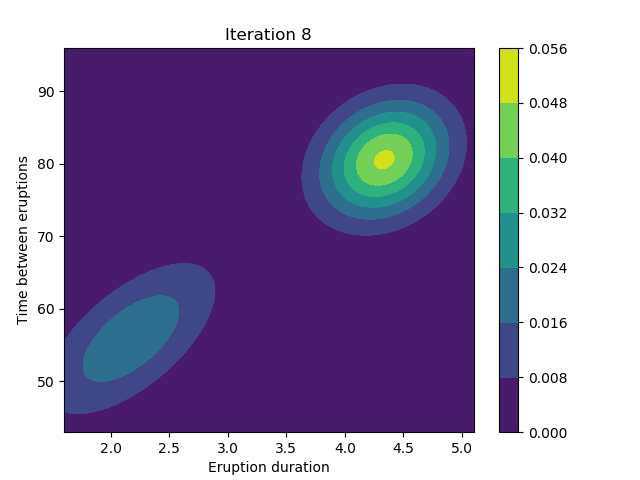
\includegraphics[width=0.33\linewidth]{contour8.png}
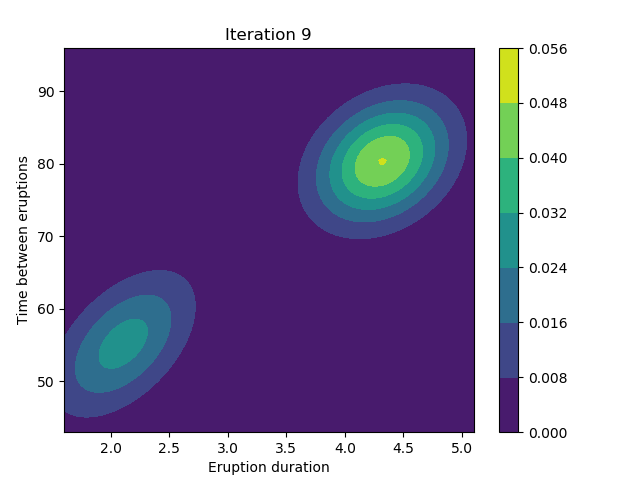
\includegraphics[width=0.33\linewidth]{contour9.png}
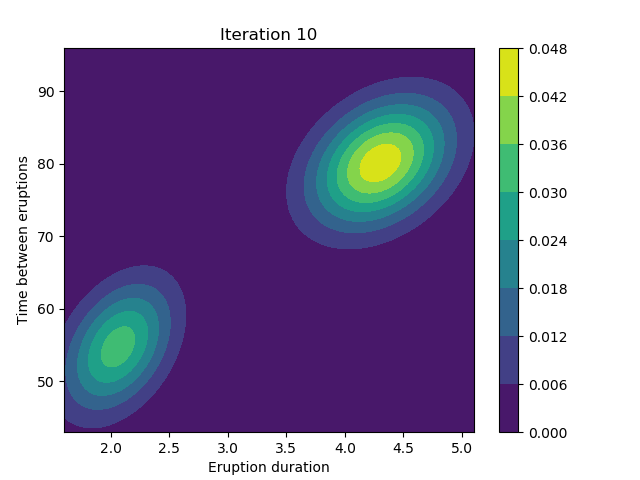
\includegraphics[width=0.33\linewidth]{contour10.png}
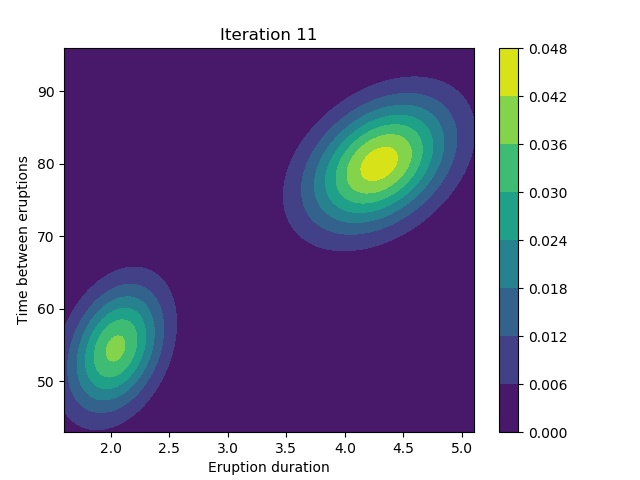
\includegraphics[width=0.33\linewidth]{contour11.png}
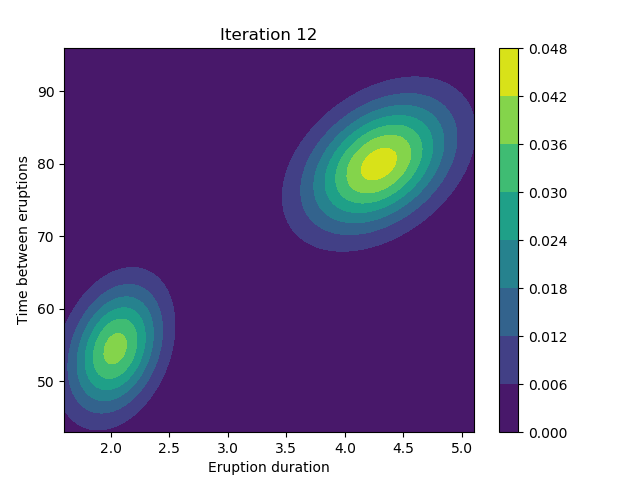
\includegraphics[width=0.33\linewidth]{contour12.png}
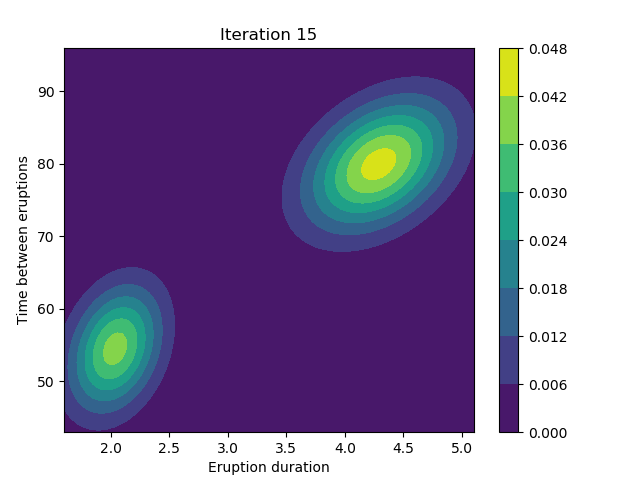
\includegraphics[width=0.33\linewidth]{contour15.png}
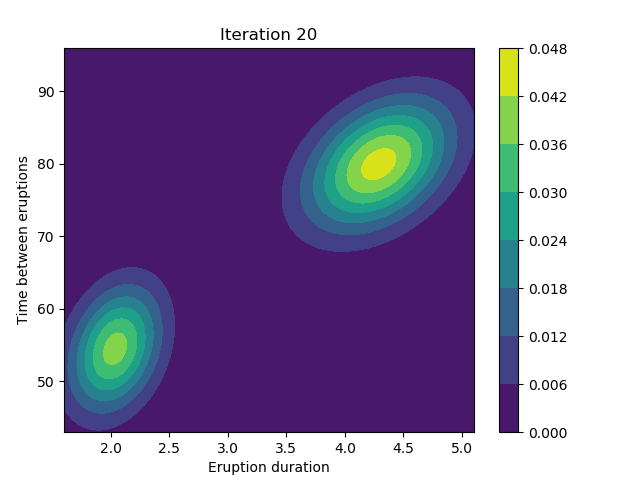
\includegraphics[width=0.33\linewidth]{contour20.png}
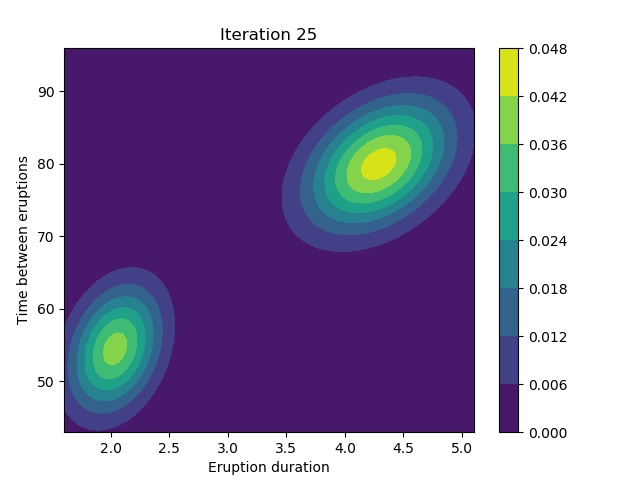
\includegraphics[width=0.33\linewidth]{contour25.png}
The next graph shows the exact positions of the means, as they are updated. This is overlaid on top of the data, and the contour plot. This helps visualise that the generated contour plots are relatively accurate with regards to the data.\\
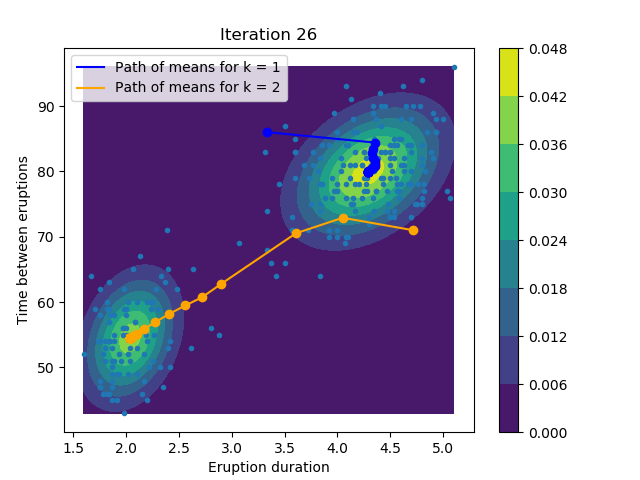
\includegraphics[width=\linewidth]{path.png}
The final graph shows the progress of the log likelihood function, over the different iterations. It makes sense intuitively, that it increases so significantly in the beginning if you also look at the previous graphs. The means and covariance matrices change significantly in the first few iterations, but rapidly converge to a point where the changes are minimal, and barely perceptible.\\
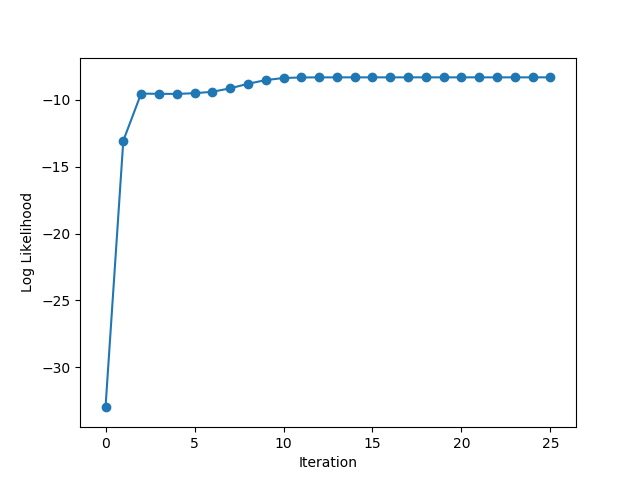
\includegraphics[width=0.75\linewidth]{log_likelihood.png}
